\documentclass{wseas}

% custom package for drawing flowcharts
\usepackage{tikz}
\usetikzlibrary{shapes.geometric, arrows}

% custom setup of how figures are rendered
\usepackage{caption}
\captionsetup[figure]{labelfont=bf,labelformat=simple,labelsep=colon,name={Fig.}}


\author{Marko Grabuloski}
\title{Enhancing Language models with RAG}  
    
\begin{document}
\twocolumn[
\begin{@twocolumnfalse}
    \maketitle
    \begin{abstract}
    This research aims to enhance the capabilities of Large Language Models
    (LLMs) using Retrieval-Augmented Generation (RAG) techniques. By
comparing the accuracy of question-answering between standard LLMs and
    those integrated with RAG systems, this study explores the potential
    improvements in performance and robustness that RAG systems can offer.
    \end{abstract}
    \begin{keywords}
    %  - Leave one blank line after the Abstract and write your Key-Words (6 - 10 words)\\
\end{keywords}

\begin{dates}
  {\break
  \color{red}
  Received: May 31, 2019. Revised: May 4, 2020. Accepted: May 22, 2020. Published: May 29, 2020
  \break(WSEAS will fill these dates in case of final acceptance, following strictly our database and possible email
  communication)}
\end{dates}
\end{@twocolumnfalse}
\vspace{2ex} 
]


\section{Topic}

Extending the capabilities of LLMs using Retrieval-Augmented Generation
techniques. Comparing the accuracy of answering questions between
standard LLM vs.~RAG LLM for different LLMs.

\section{Introduction}

LLMs are quite useful and have taken the world of AI by storm. They have
extensive usages, and we are still rediscovering what they can be used
for. However, there are some aspects that are not ideal, for example:

\begin{itemize}

\item
  \textbf{Limitation in Memory}: LLMs are trained once on a set of data.
  Once trained, they cannot answer questions or generate text on data
  they have not been trained on (problem of under-fitting and high
  bias).
\item
  \textbf{Hardware Requirements and Cost}: Running useful
  general-purpose LLM requires serious hardware capabilities, which
  comes with additional costs.
\item
  \textbf{Privacy}: Large and useful LLMs are typically run by
  companies, requiring users to send data to externally managed servers.
  This may pose problems for individual users who need to submit private
  data and for companies, especially with GDPR requirements that might
  not be satisfied.
\end{itemize}


\section{What is Retrieval augmented generation}

\emph{Retrieval-augmented generation (RAG) is an advanced artificial intelligence (AI) technique that combines information retrieval with text generation, allowing AI models to retrieve relevant information from a knowledge source and incorporate it into generated text.} (Miesle, P. no date) \cite{cite6}


The basic idea around a RAG system is extending the capabilities of an
already trained machine learning model (MLM) in particular an LLM.

One common problem in LLMs is that in order get a correct output/answer
the LLM needs to be trained on a dataset that is relevant to the
input/question. For example, asking an LLM who is the winner of 2024
euro championship will not result in a correct answer if the model is
trained before 2024. Regardless of the capabilities of the chosen LLM,
it just does not contain memory related to this information. In case
like this the LLM will need to be retrained. Different problem that
occurs in LLMs and machine models in general is that perhaps the LLM is
not powerful enough for the given task. Example for the second case is
that if a model is asked extremely difficult question, even though the
model has been trained on all the relevant data it might still not
produce correct output in case of a difficult task.

Rag systems do not suffer as much as other models from this problem,
their memory can be extended without the need for training or adding
additional parameters. The system has two types of memory:

\begin{itemize}

\item
  \textbf{Parametric memory} - refers to the knowledge in the LLM
  generative model
\item
  \textbf{Non-parametric memory} - stored in special types of databases.
  This non-parametric memory can be extended with additional knowledge
  easily and it still can be used by the LLM. \textbf{This is the core
  idea in RAG. Without any additional training new knowledge can be made
  available to the LLM.}
\end{itemize}

The RAG technique integrates a retrieval model and generative model. RAG
systems usually work around extending the capabilities of NLP(Natural
Language processing models) giving them additional memory or information
on various topics. Therefor a production RAG system in the context of
LLMs is build from 2 sub-systems:

\begin{itemize}

\item
  \textbf{Retrieval and Augmentation}
\item
  \textbf{Generative AI component} or parametric memory, it is usually
  language generation tool like LLMs
\end{itemize}

From the perspective of usage of the RAG system, the answer generation is
done in three phases:

\begin{itemize}

\item
  Phase 1 Retrieval, Knowledge retrieval, When asked a question the RAG
  retrieval system will retrieve all known information by submitting an
  appropriate query to the non-parametric memory.
\item
  Phase 2 Augmentation, with the retrieved information, a context around
  the question is created, the context should contain all information
  for answering the question.
\item
  Phase 3 Generation, The context and question will be passed to an LLM
  that will generate an answer.
\end{itemize}



\begin{figure}[htbp]
  \centering
  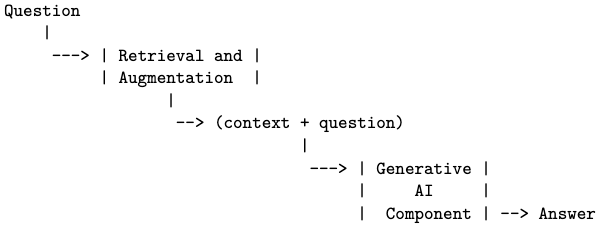
\includegraphics[width=\linewidth]{resources/v1/retrievalAndAugmentation.png}
  \caption{RAG's system retrieval and augmentation phase}
  \label{fig:rag_system_figure}
\end{figure}

%  TODO: reference image in text, try to find example in journals
% \tikzstyle{block} = [rectangle, draw, fill=blue!20, 
%     text width=10em, text centered, rounded corners, minimum height=3em]
% \tikzstyle{line} = [draw, -stealth]
% \begin{figure}[htbp]
%   \centering
%   \begin{tikzpicture}[node distance=2cm]
%     \node (question) [block] {Question};
%     \node (retrieval) [block, below of=question] {Retrieval and Augmentation};
%     \node (context) [block, below of=retrieval] {Context + Question};
%     \node (generative) [block, below of=context] {Generative AI Component};
%     \node (answer) [block, below of=generative] {Answer};

%     \path [line] (question) -- (retrieval);
%     \path [line] (retrieval) -- (context);
%     \path [line] (context) -- (generative);
%     \path [line] (generative) -- (answer);
%   \end{tikzpicture}
%   \caption{Answer generation process in a RAG system}
%   \label{fig:flowchart}
% \end{figure}



\section{Generative AI component or a LLM transformer}

The Generative AI component is an LLM transformer. Typically, the
transformer has two main components, the encoder and the decoder. The
input text is initially tokenized, meaning it is split into small
continuous lists of characters. In the next step, the model transforms
the tokens into fixed-size vectors called embeddings. In the final step,
in a so-called attention layer, an additional linear transformation on
the embeddings is performed, making them dependent on the context they
appear in. These context-dependent embeddings, also called contextual
embeddings, are the output of the encoder and the input to the decoder.
The encoder is of extreme importance in this text as it is a crucial
part of a RAG system.

\emph{Embeddings are vector representations, typically produced by a
neural network, whose main objective is to map (embed) the input media
item into a vector space, where the locality encodes the semantics of
the input} \cite{cite2}.

% TODO: add reference to the paper
% TODO: there are double : in the same sentence, this should be fixed
The decoder takes the input and generates new embeddings and again
combines the output with the embedded tokens to produce new tokens. The
vector transformation where token embeddings are transformed to
different ones to capture the context of the input text is called
attention. It is described in the paper by Vaswani et al.~(2017)
\href{https://arxiv.org/pdf/1706.03762}{Attention Is All You Need}: As a
result of the initial research paper on transformers: The LLM
transformers do not suffer from maintaining context and dependencies as
much as recurrent or convolutional networks.
Transformers can be trained significantly faster than architectures
based on recurrent or convolutional layers.

\emph{Transformers outperform the best previously reported models in
translation.} According to Vaswani et al.~\cite{cite1}

The quality of the generated text generally depends on the number of the
parameters of the model. Regardless of the quality of the output, every
LLM for a given input is expected to generate grammatically correct text
and semantically related to the input. For example if I ask even the
smallest LLM ``What is the capital of France?'' it might return ``Berlin
is the capital of France''. The answers will perhaps not be correct, but
they will contain the context of the question and grammatically correct.

\textbf{The generative component of the RAG system needs to be able for
a given input and context to generate grammatically correct sentences
related to the given context.}

\textbf{This is exactly what is achieved with the LLM transformers and
that is why they are ideal to be used in the generation phase of the RAG
system.}

\section{Retrieval System}

The retrieval system is used to store and retrieve knowledge outside the
knowledge maintained in the LLM. The knowledge here is in the form of
paragraphs, sentences, or other forms of continuous text, referred to
here as a text block. The text blocks are stored as embeddings.

This part of the system is composed of two components or modules:

\begin{itemize}

\item
  Sentence Embedding Model
\item
  Non-parametric memory
\end{itemize}

\subsection{Storing Phase}

The idea of the retrieval phase is for a given text block to create
embedding and store this embedding in the non-parametric memory.

The process is as follows:

%  TODO: use proper lists, this is probably bad
\begin{itemize}
\item
  \begin{enumerate}
  % \def\labelenumi{\arabic{enumi}.}
  % \item
    Take a text block, sentence, or paragraph.
  \end{enumerate}
\item
  \begin{enumerate}
  % \def\labelenumi{\arabic{enumi}.}
  % \setcounter{enumi}{1}
  % \item
    Passes this text to the Sentence Embedding model to get an
    embedding(dense vector).
  \end{enumerate}
\item
  \begin{enumerate}
  % \def\labelenumi{\arabic{enumi}.}
  % \setcounter{enumi}{2}
  % \item
    Stores this embedding in a non-parametric memory.
  \end{enumerate}
\end{itemize}

\begin{figure}[htbp]
  \centering
  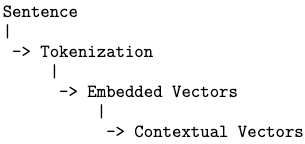
\includegraphics[width=\linewidth]{resources/v1/retrievalSystemStoringPhase.png}
  \caption{RAG retrieval system, storing phase}
  \label{fig:retrieval_system_storing_phase_figure}
\end{figure}

\subsection{Retrieval Phase}

The idea of the retrieval phase is to return all relevant information
from the non-parametric memory for a given text, query, or question.

The process is as follows:

\begin{enumerate}
\def\labelenumi{\arabic{enumi}.}
\item
  Takes input text, referred to as a query.
\item
  Passes the query text to the Sentence Embedding model to get a query
  embedding or a query dense vector.
\item
  Using the query embedding, fetches a list of related knowledge from
  the non-parametric memory.
\end{enumerate}


\begin{figure}[htbp]
  \centering
  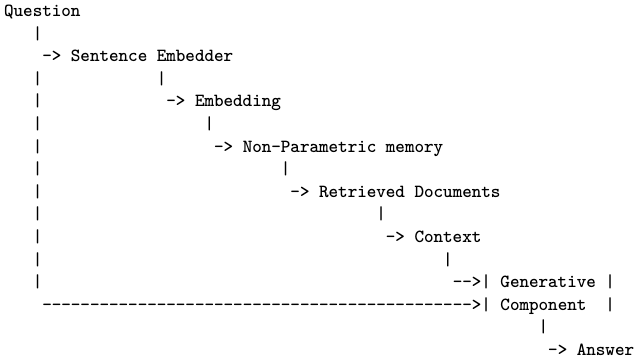
\includegraphics[width=\linewidth]{resources/v1/retrievalSystemRetreavalPhase.png} % Replace with your image path
  \caption{Siamese network with Contrastive Loss function}
  \label{fig:retrieval_system_retreaval_phase_figure}
\end{figure}

\subsubsection{Non-parametric memory - vector databases}

The non-parametric memory is usually a dense vector database. Besides
being able to store vectors, a vector database must also have the
capability to query for the k the closest vectors to a given input
vector. Like any database, fast storage and querying are important.
Ideally, these databases should be able to store data on disk to enable
horizontal scaling and data distribution, which are essential for a RAG
system to achieve scalability compared to a traditional LLM model. This
project will use the Faiss library, as it sutisfies the conditions for
vector storage and quering the k closest vectors, it laks the automatic
distributive scaling but a full DB solution is not required for the
project in this paper.

\emph{The Faiss library is dedicated to vector similarity search, a core
functionality of vector databases. Faiss is a toolkit of indexing
methods and related primitives used to search, cluster, compress, and
transform vectors} (Douze et al., 2024, p.~1) \cite{cite2}.

According to the referenced research, the Faiss database was tested with
768-dimensional ContrieverDb (name of the database from where vectors
are imported) dense vector embeddings with up to 1M vectors with 64
bytes per dimension and also with 100M vectors from DeepDb that have a
dimension of 96 and 8 bytes per dimension.

\paragraph{Popular vector databases}

In recent years, there have been significant developments in the field
of vector databases. Several new dense vector databases have emerged,
and some older databases, like NodeDB and MongoDB, have begun
incorporating vector capabilities.

Currently, (as of 2024), these are the options for dense vector storage:

\begin{itemize}

\item
  Redis Vector Similarity Search (VSS)
\item
  Pinecone - exclusively managed, closed source
\item
  Weaviate - open source
\item
  Milvus - open source
\item
  Qdrant - open source
\item
  Vespa - open source
\item
  Cloudflare Vectorize - exclusively managed, closed source
\item
  MongoDB Atlas - fully managed, closed source
\item
  Postges, pgvector - open-sourced
\end{itemize}

\emph{The previous information is taken form various blog posts (Ali, M.
2023; Cloudflare Docs, no date; Kehrer, K. 2023; Benedict, 2023;
Bratanič, T., 2023; Pondhouse Data 2023)} \cite{cite9} \cite{cite10} \cite{cite11} 
\cite{cite12} \cite{cite13} \cite{cite14} \cite{cite15} \cite{cite16}

\subsubsection{Sentence embedding models}

Sentence embedding models are derived from LLM transformer models. LLMs
transformer contains two general components, encoder and decoder. As
described in the section ``Generative AI component or a LLM
transformer'', the input of an encoder is a text, the output is a
contextual embedding.

From particular interest for the Sentence embedding models and the RAG
system is the encoder layer of the LLMs transformer.

Here is a description on how sentences are converted to embedding by an
encoder.

\textbf{LLM Transformer's encoder}

\begin{figure}[htbp]{}
  \centering
  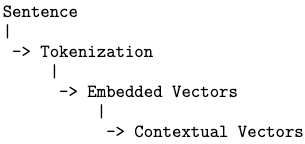
\includegraphics[width=\linewidth]{resources/v1/transformerEncoder.png}
  \caption{LLM Transformer's encoder}
  \label{fig:encoder_layer_figure}
\end{figure}

The Sentence embedding models incorporates the LLM transformers encoder
layer and adds additional layer of \emph{pooling}. This layer operates
on the token embedding and groups them in one embedding. This outputs
embedding are dependent on the context of the input text, and are called
sentence contextual embedding or sentence embedding. All the sentence
contextual embedding have the same size, and it is equal to the size of
the token embedding.


Here is a more visual description on the process of creating sentence
embedding by a Sentence embedding model:

\textbf{Sentence embedding model}

% \begin{verbatim}
% Sentence 
%  |
%   -> Tokenization
%       | 
%        -> Embedded Vectors
%            | 
%             -> Contextual Vectors
%                 | 
%                  -> | Mean Pooling            |  
%                     | Max Pooling             | 
%                     | CLS Token               |
%                     | Attention-based Pooling |
%                        | 
%                         -> Sentence embedding
% \end{verbatim}

\begin{figure}[htbp]
  \centering
  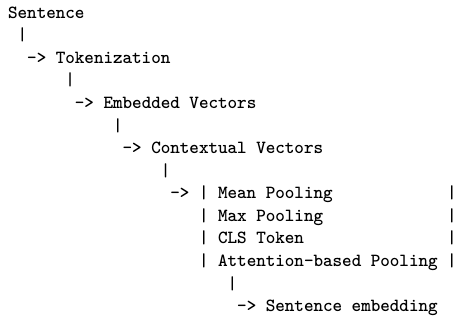
\includegraphics[width=\linewidth]{resources/v1/sentenceEmbeddingModelCreation.png}
  \caption{Sentence embedding model}
  \label{fig:sentence_embedding_model_figure}
\end{figure}

\subsubsection{Pooling}

The pooling phase involves the task of combining multiple contextual
token embeddings into one sentence embedding. The dimension of the token
embeddings is the same as the created sentence embedding. Here are some
of the popular pooling methods used in sentence embedding models:

\begin{itemize}

\item
  Mean Pooling
\item
  Max Pooling
\item
  CLS Token
\item
  Attention-based Pooling
\end{itemize}

The most representative method is Mean Pooling, which calculates an
embedding using the mean:
\begin{equation}
  meanpool(e_1, e_2, \ldots, e_n) = \frac{1}{n} \sum_{i=1}^{n} e_i
\end{equation}

According to research paper \cite{cite5} by Miesle et al.~(2023), Mean
Pooling, Max Pooling, and CLS Token are commonly used techniques.

The goal of sentence embedding models is to produce an embedding or
vector from text. As mentioned before, they are built by adding a layer
to the LLM's transformer encoder component. LLMs produce token
embeddings, while sentence embedding models produce embeddings for
entire sentences.

The requirement of the sentence embedding model is as follows:

% TODO question: should i enumerate some of the mathematical expressions, not sure since there are no formulas in this section
% TODO check what the \textless{} does, probably it is not needed
For every three blocks of text \(A\), \(P\), \(N\), the model \(SE\) is
to provide three embeddings \(SE(A)\), \(SE(P)\), \(SE(N)\),\\
such that: if \(A\) and \(P\) are semantically more similar \(A\) and
\(N\), then the distance \(distance(SE(A), SE(P))\) \textless{}
\(distance(SE(A), SE(N))\).

\textbf{The simple interpretation is that the sentence embedding model
takes a block of text and captures its meaning or semantics by
describing it as a vector.}

\textbf{This is an extremely useful feature because it allows for
representing the meaning and information of sentences in a way that
enables the measurement of semantic information.}

\subsubsection{Siamese training network and loss functions}

Up to this point, I have explained how a sentence embedding model works,
including its input and output. Even though the input and output are in
the required format, sentence embedding models are additionally trained
to meet the semantic requirements defined above.

The main issue during training is that we don't really know the exact
output for a block of text, it can be any embedding. It is the relative
distance between the embeddings that is important. Semantically close
embeddings should be closer than embeddings that have different
meanings. To solve this problem, the model is trained using a Siamese
network or a variation of the Siamese network. Initially the sentence
embedder is trained with Siamese network that conceptual contains two
copies of the same neural network. These two networks share the same
parameters. The network ends with a loss function. Popular lost
functions are contrastive loss and the triplet loss function.

\paragraph{Contrastive loss function}

Contrastive loss function uses the Siamese network. The training set
elements consist of two text blocks \(A\), \(C\) where:

\begin{itemize}

\item
  \(A\) - is called an anchor case, it is used to compare against
\item
  \(C\) - means positive or negative case, is either a text similar to
  \(A\) or a text block that is not similar to \(A\)
\end{itemize}

% \emph{Siamese network with Contrastive Loss function}

% \begin{verbatim}
%  Anchor                Positive/Negative
%   Input                      Input
%     |                          |
%  Shared Network          Shared Network 
%     |                          |
%  Anchor Embedding      Positive/Negative 
%        \                  Embedding
%         \                     /
%          \                   /
%             Contrastive Loss
%                Function
% % \end{verbatim}
% \begin{figure}[htbp]
% \begin{verbatim}
%  Anchor                Positive/Negative
%   Input                      Input
%     |                          |
%  Shared Network          Shared Network 
%     |                          |
%  Anchor Embedding      Positive/Negative 
%        \                  Embedding
%         \                     /
%          \                   /
%             Contrastive Loss
%                Function
% \end{verbatim}
% \end{figure}

\begin{figure}[htbp]
  \centering
  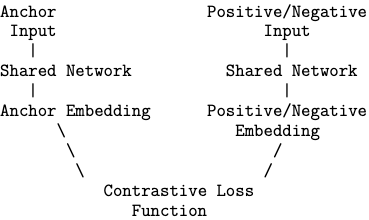
\includegraphics[width=\linewidth]{resources/v1/contrastiveLoss.png}
  \caption{Siamese network with Contrastive Loss function}
  \label{fig:contrastive_loss_function_figure}
\end{figure}

The networks end's with a contrastive loss function that is given with
the following formula:
\begin{equation} 
  Loss =  \frac{1}{2} (y*D(A,C)^2 + (1-y)*max(0,m-D(A,C))^2)
\end{equation}
In the previous function \(y\) can be 1 or 0. This is because the
network can be trained on cases with similar and dissimilar embeddings.

\begin{itemize}

\item
  Similar embeddings (y=1), the form of the loss function is: 
  \begin{equation}
    Loss = \frac{1}{2}(D(A,C))
  \end{equation}

\item
  Dissimilar embeddings (y=0), the form of the loss function is: 
  \begin{equation}
    Loss =  \frac{1}{2}(max(0,m-D(A,C))^2)
  \end{equation}
  In this case \(m\) acts as a kind of tolerance level and the
  function is triggered only for a distance bigger than \(m\).
\end{itemize}


\paragraph{Triplet Loss function}

Similarly to the Contrastive loss function training method, the triplet
loss function uses a variation of the Siamese network where instead of
two networks, three networks are used. One single test case consists of
three text blocks: \(A\), \(P\), and \(N\). * The text block \(A\) is
used for comparison and is called an anchor. * The text block \(P\) is
semantically similar to \(A\) and is called the positive case. * The
text block \(N\) is semantically different from \(A\) and \(P\) and is
called the negative case.

% \emph{Siamese network with triplet loss function}

% \begin{verbatim}
                   
% Anchor        Positive      Negative
%  Input         Input         Input
%    |             |             |
% Shared         Shared        Shared
% Network        Network       Network
%    |             |             |
% Anchor        Positive       Negative
% Embedding     Embedding     Embedding
%       \          |           /
%        \         |          /  
%         \        |         /
%          \       |        /
%           Triplet Distance
%             Loss function     
% \end{verbatim}

\begin{figure}[htbp]
  \centering
  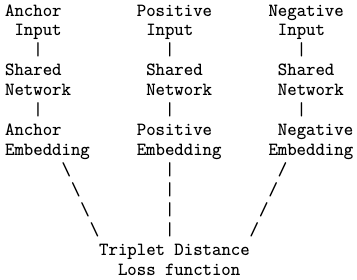
\includegraphics[width=\linewidth]{resources/v1/tripletLoss.png}
  \caption{Siamese network with triplet loss function}
  \label{fig:triplet_loss_function_figure}
\end{figure}

This Siamese network ends with a triplet distance activation function.
The function calculates the distance \(D(A,P)\) \(D(A,N)\) and is
activated if \(D(A,P)\) \textgreater{} \(D(A,N) + margin\). The
triplet function from the perspective of the Sentence embedder model is
a Loss function and its output is used for training. 

\begin{equation}
  Loss = max(0, D(A,P) - D(A,N) + margin) 
\end{equation}\cite{cite5}

If \(D(A,P) < D(A,N)\), the function returns 0 and nothing should be
adjusted for the current test case. If \(D(A,P) > D(A,N)\), then the
function returns a value greater than 0, so the model's parameters
should be adjusted to minimize this distance. The margin is there to
give a bias to the loss function and make sure that only for really
small \(D(A,P)\) compared to \(D(A,N)\) the model should not be
adjusted, but for most cases, it will be adjusted. For no adjustments to
happen, the following condition should be true:

\begin{equation}
  D(A,P) + margin < D(A,N)
\end{equation}

\subparagraph{Contrastive vs Triplet Loss function}

Both loss functions are used for training the embedder to detect
semantic similarities. The primary difference is that contrastive loss
is easier to implement in the context of generating the training set. It
requires two text chunks, whereas triplet loss requires three text
chunks. On the other hand, triplet loss often provides better results
during training. Typically, the embedder is trained twice: initially
with a contrastive loss function and later fine-tuned with a triplet
loss function.

An important point to mention is that the distance function in the
triplet or contrastive loss can vary depending on the use case of the
network. When trying to find semantic similarities, a cosine distance
between the embeddings is used, whereas in different contexts, a norm
distance like Euclidean distance can be used.

Cosine distance is based on cosine similarity, or the cosine of the
angle between the two embeddings. Cosine distance does not measure the
size of the difference between the embeddings but how similar the
direction is, as embeddings with close directions have values close to
0. Orthogonal embeddings have cosine values equal to 0, and embeddings
that are oppositely directed have cosine values close to -1. The loss
function needs to be a distance function, so just a cosine similarity
between the embeddings won't be enough since it does not satisfy the
distance requirements. That's why cosine distance is used:

% \[
% D(A, B) = 1 - \cos(\theta), 
% \]
% \[
% \mathrm{where} \ \theta \ \mathrm{is \ the \ angle \ between} \ A \ \mathrm{and} \ B
% \]
% todo check this equation with the one on top

\begin{equation}
  D(A, B) = 1 - \cos(\theta)
\end{equation}

where \(\theta\) is the angle between \(A\) and \(B\).

At this point, all the components of the sentence embedding model are
explained. A representative example of a sentence embedding model is
SBERT, which is based on the popular LLM BERT. This resource will use
SBERT as a Sentence Embedder Model.


\section{Related work}

\subsection{General RAG
systematization}

\subsubsection{Naive RAG}

Is the type of rag described in this document.

\subsubsection{Advanced RAG}

Focuses on improving the retrieval of embeddings or data. It adds
additional \textbf{pre-retrieval} and \textbf{post-retrieval} phase. In
the pre-retrieve several optimization methods are employed like: 
% TODO this should be a list
* Query
optimization * Storage optimization and retrieval * Extending the stored
data with metadata In the \textbf{post-retrieval} phase idea is to
create more usable context from the retrieved data. The data now is
re-ranked and compressed, cleaned up. This concept is derived from the
work of Gao et al.~(2023) \cite{cite4}.

\subsubsection{Modular RAG}

This type of architecture tries to split the system in to more modules
that can be independently scaled and optimized. Example: Query
Processing Module, Retriever, Re-ranking, Context Management, Generation
Module.

\subsection{Different RAG methods and
models}

\subsubsection{RAG-Sequence Model}

This type of RAG retrieves \(k\) embeddings, but unlike the standard RAG
implementation it does not use all the embeddings at the same time to
generate the answer. Before returning a token, the next token is
generated \(k\) times, meaning for every embedding one token is
generated. Then the token with the highest probability is returned. This
is done for every token.

\emph{The RAG-Sequence model uses the same retrieved document to
generate the complete sequence. Technically, it treats the retrieved
document as a single latent variable that is marginalized to get the
seq2seq probability p(y\textbar x) via a top-K approximation.
Concretely, the top K documents are retrieved using the retriever, and
the generator produces the output sequence probability for each
document, which are then marginalized} (Lewis et al., 2024, p.~3) \cite{cite3}

\subsubsection{RAG-Token Model}

Interesting research has been done using the so-called \emph{RAG-Token
Model}. The RAG technique described, initially retrieves \(k\) documents
related to the question then augments the context of the question and
sends the context and the question as an input to an LLM or the
generator. The RAG-Token Model retrieves new documents on every
generated token. Once a token is generated, the token is appended to all
previously generated tokens and this are appended to the initial
question. This results in a string of the following form ``Question +
GenerateTockenList''. This new string is then used again as an input in
the RAG, or as an input for the RAG retrieved. The process retrieves new
documents for every new generated token and uses this documents to
generate the next token. This makes sure that every new generated token
is equally dependent on the question and the non-parametric memory.

\emph{RAG-Token Model, In the RAG-Token model we can draw a different
latent document for each target token and marginalize accordingly. This
allows the generator to choose content from several documents when
producing an answer. Concretely, the top K documents are retrieved using
the retriever, and then the generator produces a distribution for the
next output token for each document, before marginalizing, and repeating
the process with the following output token} (Lewis et al., 2024, p.~3)
\cite{cite3}

\subsection{Iterative RAG}

One example is the ``Speculative RAG'' described in the paper \cite{cite18}
by (Wang 2024). Based on the question it retrieves \(N\) embeddings. The
embeddings are then clustered in \(k\) classes using K-means. From the
\(k\) clusters one embedding is selected per cluster, resulting in k
embeddings. Then the algorithm uses two LLMs so called a drafter and a
verifier. The drafter is used to generate the answer called a draft and
explanation called rational. It is important to note that not all LLMs
generate rationals. There are some that can do this, but usually the
model needs to be trained to provide the rational. The RAG-Model from
Hugginface provides explanations that can be used as a rational, also
the retrieved embeddings might be used as rationals. Once the answer and
the rational are generated, the quality of the answer and question is
measured by the verifier.

\subsubsection{Self-Consistency Score}

It gives the probability that the LLM can generate the answer and the
rational based on the question. It is given by the joint probability
formula:

\begin{equation}
  P_{sc} = P(A,B \mid Q) = P(A \mid Q) \cdot P(B \mid Q, A)
\end{equation}
  
Where:
\begin{itemize}
  \item \( A \) is the answer
  \item \( B \) is the rationale
  \item \( Q \) is the question
\end{itemize}

The value can be retreated from the LLM. It simply says what is the
probability that the answer been generated based on the question and the
probability that the rational is generated based on the question and the
answer.

\subsubsection{Self-reflection score}

It tries to determine if the rational sports the answer. For this a new
question R can be formed: Does the rational $A$ sports the answer
$B$ for the question $Q$? The new question is called a
self-reflected statement and denoted with R. Then the probability of Yes
been generated from the LLM is measured. In general, the self-reflection
score is the conditional probability of $Yes$ been generated by the
LLM given the input of a question $Q$, answer $A$, rational $B$ and self
reflected statement $R$.

Self-reflection score: 

\begin{equation}
  P_{sr} = P("Yes"|Q, A, B, R)  
\end{equation}

The process is repeated for all the clusters, and a \(p_{sr}*p_{sc}\) is
calculated. The answer with the highest \(p_{sr}*p_{sc}\) score is
picked as the most relevant, and it is the answer that is returned.


\subsection{Recursive RAG}

As any recursive algorithm it repeats its self until the results
satisfies certain criteria. In case of the retrieval, a naive RAG system
performs good when all the information required for answering the
question is in the retrieved embedding, but it fails when this
information is scattered in different embeddings. The Recursive rag
starts examine the semantically similar documents not only of the
question but also of the embeddings that are initially retrieved. With
this it tries to capture all the relevant information. The previous is
described in the paper from (Karpukhin et al.~2020; Pondhouse Data, no
date) \cite{cite16} \cite{cite17}


\section{Research methodology}

In this research, a simple RAG system will be coded. The system will be
flexible and modular enough so can use different LLMS as generators. The
system will also have a Retriever that will be able to create embeddings
based on sentences and also on paragraphs. The retriever will also
retrieve embeddings based on a question/query. All the chosen LLMs and
their appropriate RAGs will be asked three different type of Open-domain
question. This is a type of question that can't be answered with simple
yes or no and requires accessing a broad range of information to provide
an answer.

The purpose of the experiments: 1. Compare the differences between a RAG
answer and a standard LLM. 2. Assess the quality of the models for
answering different type of questions

\subsection{LLMs}

Depending on the LLMs type, three different LLM models will be used:

\begin{enumerate}
\def\labelenumi{\arabic{enumi}.}
\item
  Casual models
\item
  Question answering models
\item
  T5 - conversational models
\end{enumerate}

Regarding the model size, the experiments will be done on small LLMs
ranging from 66M up to 1.3B.


% TODO REFERENCE TABLE IN TEXT

\begin{table*}[htbp]
\centering
\caption{Model Descriptions} % Optional caption
\begin{tabular}{|p{0.3451\linewidth}|p{0.3239\linewidth}|p{0.1549\linewidth}|p{0.1761\linewidth}|}
\hline
\textbf{Model} & \textbf{Description} & \textbf{Number of Parameters} & \textbf{Type} \\
\hline
\textbf{blenderbot 90M} & Facebook AI's BlenderBot Model & 90M & Causal Model \\
\hline
\textbf{GPT-2 124M} & OpenAI's Generative Model & 124M & Causal Model \\
\hline
\textbf{GPT-Neo 125M} & EleutherAI's Generative Model & 125M & Causal Model \\
\hline
\textbf{GPT-2 Medium 355M} & OpenAI's Generative Model & 355M & Causal Model \\
\hline
\textbf{GPT-2 Large 762M} & OpenAI's Generative Model & 762M & Causal Model \\
\hline
\textbf{GPT-Neo 1.3B} & EleutherAI's Generative Model & 1.3B & Causal Model \\
\hline
\textbf{DistilBERT} & Hugging Face's Optimized BERT for QA & 66M & Question Answering Model \\
\hline
\textbf{roberta-base} & Facebook AI's Optimized BERT for QA & 125M & Question Answering Model \\
\hline
\textbf{bert-large-uncased-whole-word-masking-finetuned-squad} & Google's NLU Model for QA & 340M & Question Answering Model \\
\hline
\textbf{T5 Base 220M} & Google's Text-to-Text Transfer Transformer & 220M & T5 - Conversational Model \\
\hline
\textbf{T5 Large 770M} & Google's Text-to-Text Transfer Transformer & 770M & T5 - Conversational Model \\
\hline
\end{tabular}
\end{table*}
  

\emph{For comparison, the currently used production ChatGPT 3.5,
according to ChatGPT, has a size of around 175B. ChatGPT 4.0 has not
exposed any information about the number of parameters or architecture.
Most probably, both models employ the RAG technique to improve their
performance.}

It is important to point out that the causal models are not trained for
answering questions but for generating text based on input. Running a
RAG around causal LLMs will give an idea of how powerful a RAG system
can be. The question-answering models are more suitable for usage in a
RAG system. They extract the continuous character set in the context
that has the highest probability of being an answer given a specific
question. The T5 models are conversational models, and although they are
not specifically trained to answer questions, they are trained to
maintain a conversation and should outperform the causal and
question-answering LLMs.

\subsection{Questions}

The questions asked and their types are:

\begin{enumerate}
\def\labelenumi{\arabic{enumi}.}
\item
  Fact-based question - ``How tall is the Pyramid of Giza?''
\item
  List-based question - ``What materials were used in constructing the
  Great Wall of China?''
\item
  Synthesis-based Fact question - ``Which famous structures were either
  designed or structurally influenced by Gustave Eiffel?''
\end{enumerate}

The ``Synthesis-based Fact'' question is a type of question where the
answer needs to be derived from more than one retrieved fact. Unlike the
other questions, where the answer is directly contained in the
embedding, correctly answering the synthesis-based fact question implies
that the retrieval system correctly mapped and retrieved the embeddings,
and that the LLM is capable of drawing conclusions based on several
facts.


\subsection{Retrieval and
augmentation}

There will be 3 types of RAG augmentation, in this text called
retrieval:

\begin{itemize}

\item
  Retrieval of one sentence, will create a context for the question from
  one sentence using a facts sentence based database.
\item
  Retrieval of one paragraph, will create a context for the question
  from one paragraph using a facts sentence based database.
\item
  Retrieval of three paragraphs, will create a context for the question
  from three paragraphs using a facts paragraph based database. The
  database for the sentences and paragraphs are created from two files
  containing semantically correct but not necessarily related sentences
  and paragraphs.
\end{itemize}

\subsection{RAG solution}

The RAG system will be a manual solution, not an existing RAG system.
The idea is to show that even a simple RAG system can extend the
capabilities of the LLM.

\subsection{Sentence Embedder}

For sentence embedder a SBART based embedder will be used:

\begin{verbatim}
sentence_transformers import SentenceTransformer
\end{verbatim}

\subsubsection{Non-Parametric library}

For non-parametric library \texttt{faiss} will be used, it is more than
enough to handle this experiment.

\subsubsection{Environment}

Jupyter notebook.

\subsubsection{Hardware}

For the particular reasons an open sourced LLMs will be used that can be
run locally on the pc. The chosen hardware is a m3 processor with 36GB
of RAM.

\subsubsection{Experiments definition}

In total five experiments will be performed.

% TODO REFERENCE TABLE IN TEXT

\begin{table*}[htbp]
\centering
\begin{tabular}{|p{0.15\linewidth}|p{0.35\linewidth}|p{0.25\linewidth}|p{0.20\linewidth}|}
\hline
\textbf{Experiment} & \textbf{Question Type} & \textbf{Augmentation Type} & \textbf{Augmentations} \\ \hline
1 & Fact-based question & Sentence & 1 \\ \hline
2 & List-based question & Sentence & 1 \\ \hline
3 & Fact-based question & Paragraph & 1 \\ \hline
4 & List-based question & Paragraph & 1 \\ \hline
5 & Synthesis-based Fact question & Paragraph & 3 \\ \hline
\end{tabular}
\caption{Experiment Table}
\end{table*}

    

\section{Results and discussion}

\subsection{Experiment 1: Fact-based Question - ``How tall is the
Pyramid of
Giza?''}

\subsubsection{Experiment Description}
In this experiment, various language models were tested to answer the
fact-based question: ``How tall is the Pyramid of Giza?''. The
experiment parameters are as follows:

\begin{itemize}

\item
  \textbf{Question Type}: Fact-based
\item
  \textbf{Question}: ``How tall is the Pyramid of Giza?''
\item
  \textbf{Retrieval Type}: Sentence retrieval
\item
  \textbf{Number of Retrievals}: 1
\end{itemize}

\subsubsection{Causal Models}

% TODO REFERENCE TABLE IN TEXT

\begin{table*}[htbp]
\centering
\begin{tabular}{|p{0.10\linewidth}|p{0.48\linewidth}|p{0.42\linewidth}|}
\hline
\textbf{LLM} & \textbf{LLM Answer} & \textbf{RAG Answer} \\ \hline
facebook blenderbot-90M & balkicker mutations mutations pment mutations mutations mutations kicker fiers eston eston eston eres bender eston \ldots{} & lease willis lease mative mative lease willis mative lease lease lease willis \ldots{} \\ \hline
gpt2 & The Pyramid of Giza is the tallest building in Egypt. The Pyramid of Giza is located in the Giza Plateau \ldots{} & The Great Pyramid of Giza is the largest and oldest of the three pyramids, standing at 146.6 meters \ldots{} \\ \hline
EleutherAI gpt-neo-125M & The Pyramid of Giza is the tallest pyramid in the world. It was completed in the 13th century AD \ldots{} & The Pyramid of Giza is the largest and oldest of the three pyramids, standing at 146.6 meters \ldots{} \\ \hline
gpt2-medium & The Pyramid of Giza is the tallest structure in Egypt. It is 1,068 feet tall, and is one of the largest pyramids \ldots{} & The Pyramid of Giza is the largest and oldest of the three pyramids, standing at 146.6 meters \ldots{} \\ \hline
gpt2-large & The Pyramid of Giza is the tallest structure in the world. How tall is the Taj Mahal? \ldots{} & The Great Pyramid of Giza is the largest and oldest of the three pyramids, standing at 146.6 meters \ldots{} \\ \hline
EleutherAI gpt-neo-1.3B & The Pyramid of Giza is one of the Seven Wonders of the Ancient World. It is one of the Seven Wonders of the Modern World \ldots{} & The pyramid of Giza, also known as the Pyramid of Khufu\ldots{} and oldest of the three pyramids, standing at 146.6 meters \ldots{} \\ \hline
\end{tabular}
\caption{Comparison of LLM and RAG Answers}
\end{table*}

In all the cases the casual models generated a wrong LLM answer. Except
the \texttt{facebook/blenderbot-90M} they all generated grammatically
correct sentences. Concerning the RAG answers, all of them generated a
correct RAG answer except the \texttt{facebook/blenderbot-90M}. This is
an amazing result since without any additional training or tuning, the
models when using a RAG approach were able to generate a correct answer.
Taking in to consideration the parameters the smallest model that give a
correct answer was GPT2 with 90M.


\subsubsection{QA Models}

% TODO REFERENCE TABLE IN TEXT

\begin{table*}[htbp]
\centering
\begin{tabular}{|p{0.37\linewidth}|p{0.40\linewidth}|p{0.23\linewidth}|}
\hline
\textbf{LLM} & \textbf{LLM Answer} & \textbf{RAG Answer} \\ \hline
distilbert-base-uncased-distilled-squad\_66M & how tall is the pyramid of giza? {[}SEP{]} & 146.6 meters \\ \hline
deepset roberta-base-squad2\_125M &  & 146.6 meters (481 feet) \\ \hline
bert-large-uncased-whole-word-masking-finetuned-squad\_340M & tall & 146.6 meters \\ \hline
\end{tabular}
\caption{Comparison of LLM and RAG Answers on the Pyramid of Giza Height}
\end{table*}

The QA models are also answered correctly. Compared to the casual LLMs
RAG generated answer, here the models perform better as a model of 66M
was able to answer the question correctly. The generated LLM answer was
wrong for every model.

\subsubsection{T5 Models}

% TODO REFERENCE TABLE IN TEXT
\begin{table*}[htbp]
\centering
\begin{tabular}{|l|l|l|}
\hline
\textbf{LLM} & \textbf{LLM Answer} & \textbf{RAG Answer} \\ \hline
t5-base\_220M & None & 146.6 meters (481 feet) \\ \hline
t5-large\_770M & False & 140 meters (481 feet) \\ \hline
\end{tabular}
\caption{Comparison of LLM and RAG Answers on the Pyramid of Giza Height}
\end{table*}

The T5 models RAG generated answer is also correct for all the models.
At this point they perform the quality of the answer is on the same
level of the QA models and Casual models. But the models a bigger than
the QA models.

Conclusion: Given the size of the models the QA models are most
appropriate for answering Fact-based Question.


\subsection{Experiment 2: List-based Question - ``What materials were
used in constructing the Great Wall of
China?''}

\subsubsection{Experiment Description}

In this experiment, various language models were tested to answer the
list-based question: ``What materials were used in constructing the
Great Wall of China?''. The experiment parameters are as follows:

\begin{itemize}

\item
  \textbf{Question Type}: List-based Question
\item
  \textbf{Question}: ``What materials were used in constructing the
  Great Wall of China?''
\item
  \textbf{Retrieval Type}: Sentence retrieval
\item
  \textbf{Number of Retrievals}: 1
\end{itemize}

\subsubsection{Causal Models}

% TODO REFERENCE TABLE IN TEXT

\begin{table*}[htbp]
\centering
\begin{tabular}{|p{0.15\linewidth}|p{0.4\linewidth}|p{0.4\linewidth}|}
\hline
\textbf{LLM} & \textbf{LLM Answer} & \textbf{RAG Answer} \\ \hline
facebook blenderbot-90M & pos sitter sitter drip ba ba ba le diving ba ba bee ba ba da ba ba cats ba ba table da ba da disc ba ba orba da da prba ba prda da \textbf{end} & scibal pubalfatty composition asses sciscifatty fatty bee pumubee bee mubee zarbalpuscibal mutbal bee bal composition fatty composition fatty bee bal strip scimutcomposition \textbf{end} \\ \hline
gpt2 & The Great Wall of China is the largest in the world, and is the largest city in the world. It is the largest city in the world. It is the largest city in & The Great Wall of China is made of various materials, including stone, brick, tamped earth, and wood. The Great Wall of China was built by the People's Republic of \ldots{} \\ \hline
EleutherAI gpt-neo-125M & The Great Wall of China was constructed by the Chinese government in the 17th century, and is known as the Great Wall of China \ldots{} & The Great Wall of China is made of various materials, including stone, brick, tamped earth, and wood. Answer What materials were used in constructing the Great Wall of China? \\ \hline
gpt2-medium & The Great Wall of China was built by the Ming Dynasty (1644-1911). The Great Wall was constructed of a combination of stone, wood, and metal \ldots{} & 'Answer The Great Wall of China was built of various materials, including stone, brick, tamped earth, and wood. The Great Wall of China was constructed of various materials, including stone \ldots{} \\ \hline
gpt2-large & The Great Wall of China was built by the Qin Dynasty (221-206 B.C.), which lasted from 221 to 206 B.C. \ldots{} & 'The Great Wall of China is made of various materials, including stone, brick, tamped earth, and wood.'Answer What materials were used in constructing the Great Wall of China? \\ \hline
EleutherAI gpt-neo-1.3B & The Great Wall of China was constructed using many different types of materials, including wood, stone, brick, clay, and iron \ldots{} & The Great Wall of China is made of various materials, including stone, brick, tamped earth, and wood. \\ \hline
\end{tabular}
\caption{Comparison of LLM and RAG Answers for the Great Wall of China}
\end{table*}


In all cases, the causal models generated incorrect or irrelevant LLM
answers. The RAG approach, however, performed significantly better, with
all models providing correct information about the materials used in
constructing the Great Wall of China. This demonstrates the
effectiveness of RAG in generating accurate answers even when the base
model's output is flawed.

\subsubsection{QA Models}


% TODO REFERENCE TABLE IN TEXT
\begin{table*}[htbp]
\centering
\begin{tabular}{|p{0.25\linewidth}|p{0.35\linewidth}|p{0.35\linewidth}|}
\hline
\textbf{LLM} & \textbf{LLM Answer} & \textbf{RAG Answer} \\ \hline
distilbert-base-uncased-distilled-squad\_66M & what materials were used in constructing the great wall of china? {[}SEP{]} & stone, brick, tamped earth, and wood \\ \hline
deepset roberta-base-squad2\_125M & & stone, brick, tamped earth, and wood \\ \hline
bert-large-uncased-whole-word-masking-finetuned-squad\_340M & & stone, brick, tamped earth, and wood \\ \hline
\end{tabular}
\caption{Comparison of LLM and RAG Answers for materials used in constructing the Great Wall of China}
\end{table*}


The QA models performed well in generating correct RAG answers,
accurately listing the materials used in constructing the Great Wall of
China. Similar to the first experiment, the generated LLM answers were
incorrect, but the RAG system compensated for this by providing correct
and relevant answers, showing its strength in retrieving and presenting
accurate information.

\subsubsection{T5 Models}

%  TODO reference table in text
\begin{table*}[htbp]
\centering
\begin{tabular}{|p{0.25\linewidth}|p{0.35\linewidth}|p{0.35\linewidth}|}
\hline
\textbf{LLM} & \textbf{LLM Answer} & \textbf{RAG Answer} \\ \hline
t5-base\_220M & None & stone, brick, tamped earth, and wood \\ \hline
t5-large\_770M & False & stone, brick, tamped earth, and wood \\ \hline
\end{tabular}
\caption{Comparison of LLM and RAG Answers for materials used in constructing the Great Wall of China}
\end{table*}


The T5 models also demonstrated strong performance in the RAG approach,
correctly listing the materials used in constructing the Great Wall of
China. However, like the other models, their direct LLM answers were
inaccurate or non-informative, further highlighting the importance of
RAG in ensuring accurate output.

\textbf{Conclusion:}

Given the size of the models the QA models are most appropriate for
answering List-based Question.


\subsection{Experiment 3: Fact-based Question - ``How tall is the
Pyramid of
Giza?''}

\subsubsection{Experiment Description}

In this experiment, various language models were tested to answer the
fact-based question: ``How tall is the Pyramid of Giza?'' using
paragraph retrieval with one retrieved document. Storing paragraphs is
more efficient than storing sentences, as the size of the database will
be smaller and paragraphs hold more context and information than the
sentences. The experiment parameters are as follows:

\begin{itemize}

\item
  \textbf{Question Type}: Fact-based Question
\item
  \textbf{Question}: ``How tall is the Pyramid of Giza?''
\item
  \textbf{Retrieval Type}: Paragraph retrieval
\item
  \textbf{Number of Retrievals}: 1
\end{itemize}

\subsubsection{Causal Models}

% TODO REFERENCE TABLE IN TEXT
\begin{table*}[htbp]
\centering
\begin{tabular}{|p{0.15\linewidth}|p{0.4\linewidth}|p{0.4\linewidth}|}
\hline
\textbf{LLM} & \textbf{LLM Answer} & \textbf{RAG Answer} \\ \hline
facebook blenderbot-90M & pickbalfiers fiers predators mutations bender mutations mutations eston mutations eston predators kicker mutations mutations predators mutations pment eston eston eston trout mutations fiers eston eston bender eston eston kicker eston eston fiers eston joreston \textbf{end} & design mutpuwillis willis design lease orpotbee willis potpotdistribution fatty fatty composition lease mutfatty fatty willis strip spy lease willis distribution willis strip distribution mutdraft mutpupumutspy \textbf{end} \\ \hline
gpt2 & The Pyramid of Giza is the tallest building in the world. It is located in the northern part of the country of Egypt. It is one of the tallest buildings in the world & The Great Pyramid of Giza is the tallest man-made structure in the world for over 3,800 years until the construction of Lincoln Cathedral in England in 1311. The Sphinx is \\ \hline
EleutherAI gpt-neo-125M & How tall is the Pyramid of Giza? How tall is the Pyramid of Giza? How tall is the Pyramid of Giza? How tall is & The Great Pyramid of Giza was the tallest man-made structure in the world for over 3,800 years until the construction of Lincoln Cathedral in England in 1311. The Great \\ \hline
gpt2-medium & The Pyramid of Giza, also known as the Great Pyramid of Giza or Pyramid of the Sun, is one of the world's largest pyramids. It was built in Egypt & The Pyramid of Giza is the tallest man-made structure in the world for over 3,800 years until the construction of Lincoln Cathedral in England in 1311. The Sphinx, \\ \hline
gpt2-large & The Pyramid of Giza is believed to be the tallest structure in the world. The Pyramid of Giza is located in Egypt. The Pyramid of Giza was built between & The height of the Great Pyramid of Giza is 146.6 meters (481 feet). This is the tallest man-made structure in the world for over 3,800 years. The \\ \hline
EleutherAI gpt-neo-1.3B & This is a question that has been asked many times, but the answer is not always so simple. Some of the tallest buildings in the world are located in the United States, and & The Pyramids of Giza are the only remaining structure of the Seven Wonders of the Ancient World. The Great Pyramid of Giza, also known as the Pyramid of Khuf \\ \hline
\end{tabular}
\caption{Comparison of LLM and RAG Answers for facts about the Pyramid of Giza}
\end{table*}


In this experiment, the causal models generally provided incorrect or
nonsensical LLM answers. However, the RAG approach performed
significantly better, producing correct answers by accurately retrieving
and presenting the relevant information from the paragraph.

\subsubsection{QA Models}
% TODO REFERENCE TABLE IN TEXT
\begin{table*}[htbp]
\centering
\begin{tabular}{|p{0.3\linewidth}|p{0.4\linewidth}|p{0.2\linewidth}|}
\hline
\textbf{LLM} & \textbf{LLM Answer} & \textbf{RAG Answer} \\ \hline
distilbert-base-uncased-distilled-squad\_66M & how tall is the pyramid of giza? {[}SEP{]} & 146.6 meters \\ \hline
deepset roberta-base-squad2\_125M &  & 146.6 meters (481 feet) \\ \hline
bert-large-uncased-whole-word-masking-finetuned-squad\_340M & tall & 146.6 meters \\ \hline
\end{tabular}
\caption{Comparison of LLM and RAG Answers regarding the height of the Pyramid of Giza}
\end{table*}

The QA models continued to perform well, with the RAG approach providing
correct and relevant answers. Despite the direct LLM answers being
incorrect, the RAG system ensured accurate information was retrieved and
presented.

\subsubsection{T5 Models}

% TODO REFERENCE TABLE IN TEXT

\begin{table*}[htbp]
\centering
\begin{tabular}{|p{0.3\linewidth}|p{0.4\linewidth}|p{0.2\linewidth}|}
\hline
\textbf{LLM} & \textbf{LLM Answer} & \textbf{RAG Answer} \\ \hline
t5-base\_220M & None & 146.6 meters (481 feet) \\ \hline
t5-large\_770M & False & 146.6 meters \\ \hline
\end{tabular}
\caption{Comparison of LLM and RAG Answers regarding the height of the Pyramid of Giza}
\end{table*}


The T5 models also demonstrated strong performance in the RAG approach,
consistently providing the correct height of the Pyramid of Giza. As
seen in previous experiments, the direct LLM answers were inaccurate,
underscoring the importance of using RAG for accurate outputs.

\textbf{Conclusion:}

The QA models and T5 models were particularly efficient, consistently
providing the correct height of the Pyramid of Giza. Given the size of
the models, the most efficient for answering Fact-based Question with
one paragraph retrieval are the QA models.

\subsection{Experiment 4: List-based Question - ``What materials were
used in constructing the Great Wall of
China?''}

\subsubsection{Experiment Description}

In this experiment, various language models were tested to answer the
list-based question: ``What materials were used in constructing the
Great Wall of China?'' using paragraph retrieval with one retrieved
document. The experiment parameters are as follows:

\begin{itemize}

\item
  \textbf{Question Type}: List-based Question
\item
  \textbf{Question}: ``What materials were used in constructing the
  Great Wall of China?''
\item
  \textbf{Retrieval Type}: Paragraph retrieval
\item
  \textbf{Number of Retrievals}: 1
\end{itemize}

\subsubsection{Causal Models}
% TODO REFERENCE TABLE IN TEXT

\begin{table*}[htbp]
\centering
\caption{Comparison of LLM and RAG Answers for Various Models} % Optional caption
\begin{tabular}{|p{0.0977\linewidth}|p{0.4805\linewidth}|p{0.4219\linewidth}|}
\hline
\textbf{LLM} & \textbf{LLM Answer} & \textbf{RAG Answer} \\
\hline
facebook blenderbot-90M & horn ba ba squba ba ba da ba ba bal ba ba phba ba eling ba ba sheet ba ba itba da phth ba ba muba da da audprba da \textbf{end} & potpotscistrip scipotorscizarpotdistribution scipotstrip strip cupotstrip sciscistrip potsciscibee qpotstrip cuqstrip potqsciqstrip sci\_\_end\_\_ \\
\hline
gpt2 & There are many materials that were used in the construction of the Great Wall of China, but only a few were used for the construction of the Great Wall of China \ldots{} & The Great Wall of China was built to protect against invasions from northern tribes. The Great Wall of China is made of various materials, including stone, brick, tamped earth \ldots{} \\
\hline
EleutherAI gpt-neo-125M & The Great Wall of China was built by the Chinese government during the reign of the Qing dynasty \ldots{} & The Great Wall of China is over 13,000 miles long. Construction of the Great Wall of China began in the 7th century BC. The Great Wall of China was \ldots{} \\
\hline
gpt2-medium & The Great Wall of China was constructed by a team of Chinese engineers, engineers, and architects \ldots{} & The Great Wall of China was constructed of various materials, including stone, brick, tamped earth, and wood. The height of the Great Wall of China varies, with the tallest \ldots{} \\
\hline
gpt2-large & The Great Wall of China was constructed by the Han Dynasty (206 BC -- 220 AD) \ldots{} & The Great Wall of China is made of various materials, including stone, brick, tamped earth, and wood. The height of the Great Wall of China varies, with the tallest sections \ldots{} \\
\hline
EleutherAI gpt-neo-1.3B & The Great Wall of China is one of the most famous examples of ancient Chinese architecture \ldots{} & The Great Wall of China is made of various materials, including stone, brick, tamped earth, and wood. The height of the Great Wall of China varies, with the tallest \ldots{} \\
\hline
\end{tabular}
\end{table*}


In this experiment, the causal models generally provided incorrect or
nonsensical LLM answers. The RAG approach, however, showed improvement,
with more accurate information being retrieved and presented. Despite
this, the answers still lacked consistency in listing all the materials
used in the construction of the Great Wall of China.

\subsubsection{QA Models}

\begin{table*}[htbp]
\centering
\caption{Comparison of LLM and RAG Answers} % Optional caption
\begin{tabular}{p{0.3714\linewidth} p{0.4000\linewidth} p{0.2286\linewidth}}
\toprule
\textbf{LLM} & \textbf{LLM Answer} & \textbf{RAG Answer} \\
\midrule
distilbert-base-uncased-distilled-squad\_66M & what materials were used in constructing the great wall of china? {[}SEP{]} & stone, brick, tamped earth, and wood \\
deepset roberta-base-squad2\_125M & & stone, brick, tamped earth, and wood \\
bert-large-uncased-whole-word-masking-finetuned-squad\_340M & & stone, brick, tamped earth, and wood \\
\bottomrule
\end{tabular}
\end{table*}
  

The QA models performed exceptionally well in generating correct RAG
answers, accurately listing the materials used in constructing the Great
Wall of China. The direct LLM answers were not particularly useful, but
the RAG system effectively retrieved and presented the necessary
information.

\subsubsection{T5 Models}

\begin{table*}[htbp]
\centering
\caption{Comparison of LLM and RAG Answers} % Optional caption for the table
\begin{tabular}{p{0.3714\linewidth} p{0.4000\linewidth} p{0.2286\linewidth}}
\toprule
\textbf{LLM} & \textbf{LLM Answer} & \textbf{RAG Answer} \\
\midrule
distilbert-base-uncased-distilled-squad\_66M & what materials were used in constructing the great wall of china? {[}SEP{]} & stone, brick, tamped earth, and wood \\
deepset roberta-base-squad2\_125M & & stone, brick, tamped earth, and wood \\
bert-large-uncased-whole-word-masking-finetuned-squad\_340M & & stone, brick, tamped earth, and wood \\
\bottomrule
\end{tabular}
\end{table*}

The T5 models also performed well in the RAG approach, consistently
providing the correct list of materials used in constructing the Great
Wall of China. Similar to other models, the direct LLM answers were
inaccurate or non-informative, but the RAG system ensured accurate
output.

\textbf{Conclusion:}

The QA models proved to be the most efficient for answering list-based
questions with paragraph retrievals. Their performance in generating
accurate RAG answers highlights their suitability for RAG-based
solutions, especially when detailed and precise information is required.
Given the size and efficiency, the QA models are the best choice for
implementing a RAG solution in this context.


\subsection{Experiment 5: Synthesis-based Question - ``Which famous
structures, both designed or structurally influenced by Gustave
Eiffel?''}

\subsubsection{Experiment Description}

In this experiment, various language models were tested to answer the
synthesis-based question: ``Which famous structures, both designed or
structurally influenced by Gustave Eiffel?'' using paragraph retrieval
with three retrieved documents. The experiment parameters are as
follows:

\begin{itemize}

\item
  \textbf{Question Type}: Synthesis-based Question
\item
  \textbf{Question}: ``Which famous structures, both designed or
  structurally influenced by Gustave Eiffel?''
\item
  \textbf{Retrieval Type}: Paragraph retrieval
\item
  \textbf{Number of Retrievals}: 3
\end{itemize}

The synthesis-based question require that several facts are take in to
consideration inorder to answer the quiestion. In this case the
retreaver will need provide the generator several paragraphs with
information on Gustave Eiffel. Then the LLM needs combine the facts in
to conclusion and generate the answer.

\subsubsection{Causal Models}

% TODO REFERENCE TABLE IN TEXT

\begin{table*}[htbp]
\centering
\caption{Comparison of LLM and RAG Answers for Various Models} % Optional caption
\begin{tabular}{|p{0.0977\linewidth}|p{0.4805\linewidth}|p{0.4219\linewidth}|}
\hline
\textbf{LLM} & \textbf{LLM Answer} & \textbf{RAG Answer} \\
\hline
facebook blenderbot-90M & etically ication ix belle ication belle ication judgment ication belle le tacication belle conception ication le le belle ication planted le tacdden ication tacication judge ix ication le ication judge belle ication ication le \textbf{end} & Error generating text for facebook blenderbot-90M \\
\hline
gpt2 & They're not, but it's hard not to feel a twinge of nostalgia for them \ldots{} & The Eiffel Tower is located in Paris, France. The Eiffel Tower was completed in 1889. The Eiffel Tower was painted every seven years to prevent it \ldots{} \\
\hline
EleutherAI gpt-neo-125M & This article is part of a series of articles that explore Gustave Eiffel's influence on architecture and design \ldots{} & The Colosseum was completed in AD 80. The Colosseum was designed by Gustave Eiffel, who also designed the Eiffel Tower. \\
\hline
gpt2-medium & There are many, many, many. Some of the most famous of them are: The Eiffel Tower, Paris \ldots{} & The Eiffel Tower is located in Paris, France. The Eiffel Tower was completed in 1889. The Eiffel Tower is 324 meters tall. The Eiffel Tower was designed by Gustave Eiffel. \\
\hline
gpt2-large & The Louvre, Paris, France The Eiffel Tower, Paris, France The Eiffel Tower, Paris, France \ldots{} & The Eiffel Tower is located in Paris, France. The Eiffel Tower is 324 meters tall. The Eiffel Tower was designed by Gustave Eiffel. \\
\hline
EleutherAI gpt-neo-1.3B & The Eiffel Tower in Paris. The Eiffel Tower in Paris. The Eiffel Tower in Paris \ldots{} & The Eiffel Tower is located in Paris, France. The Eiffel Tower was completed in 1889. The Eiffel Tower is 324 meters tall. \\
\hline
\end{tabular}
\end{table*}

In this experiment, the causal models struggled to produce accurate or
relevant LLM answers. The RAG approach helped improve the accuracy but
was still limited, with most models failing to provide a comprehensive
list of structures designed or influenced by Gustave Eiffel. The answers
often lacked synthesis, indicating that causal models might not be the
best choice for complex synthesis-based questions.


\subsubsection{QA Models}

% REFERENCE TABLE IN TEXT
\begin{table*}[htbp]
\centering
\caption{Comparison of LLM and RAG Answers for Various Models} % Optional caption
\begin{tabular}{|p{0.3714\linewidth}|p{0.4000\linewidth}|p{0.2286\linewidth}|}
\hline
\textbf{LLM} & \textbf{LLM Answer} & \textbf{RAG Answer} \\
\hline
distilbert-base-uncased-distilled-squad\_66M & which famous structures, both designed or structurally influenced by Gustave Eiffel? {[}SEP{]} & statue of liberty \\
\hline
deepset roberta-base-squad2\_125M & & \\
\hline
bert-large-uncased-whole-word-masking-finetuned-squad\_340M & & statue of liberty \\
\hline
\end{tabular}
\end{table*}


The QA models had mixed performance in this experiment. While the direct
LLM answers were often uninformative, the RAG answers did manage to
identify at least one structure associated with Gustave Eiffel, but they
lacked completeness. The synthesis required for this question appeared
challenging for these models.

\subsubsection{T5 Models}

% Referece table in text
\begin{table*}[htbp]
\centering
\caption{Comparison of LLM and RAG Answers for T5 Models} % Optional caption
\begin{tabular}{|p{0.3714\linewidth}|p{0.4000\linewidth}|p{0.2286\linewidth}|}
\hline
\textbf{LLM} & \textbf{LLM Answer} & \textbf{RAG Answer} \\
\hline
t5-base\_220M & None & The Eiffel Tower \\
\hline
t5-large\_770M & False & Eiffel Tower and The Statue of Liberty \\
\hline
\end{tabular}
\end{table*}


The T5 models performed relatively well in the RAG approach, with the
larger model (T5-large) being able to correctly list both the Eiffel
Tower and the Statue of Liberty as structures associated with Gustave
Eiffel. This highlights the potential of T5 models in synthesis-based
tasks, especially when more complex reasoning is required.

\textbf{Conclusion:}

For synthesis-based questions, the T5 models, particularly the larger
variant, demonstrated the most potential in the RAG approach,
successfully identifying multiple structures associated with Gustave
Eiffel. Although the QA models could partially answer the question, they
struggled with the complexity of synthesizing information from multiple
documents. The causal models, even with RAG, were not able to handle
this task effectively. Therefore, T5 models are the best choice for
RAG-based solutions when dealing with synthesis-based questions.


\section{Conclusion}

This text demonstrates through experimentation that Retrieval-Augmented
Generation (RAG) systems effectively address some of the most
significant challenges faced by Large Language Models (LLMs) and other
models with parametric memory. Compared to models solely relying on
parametric memory, RAG systems offer several advantages:

\begin{itemize}

\item
  \textbf{Horizontally Scalable}: RAG systems can efficiently scale by
  distributing the retrieval process across multiple nodes, allowing for
  handling larger datasets and more complex queries.
\item
  \textbf{Distributive}: The modular nature of RAG systems enables
  distribution of tasks across different components, enhancing
  robustness and flexibility.
\item
  \textbf{Mitigates High Bias}: By integrating external knowledge
  retrieval, RAG systems reduce the need for extremely large models with
  numerous parameters, thus avoiding issues related to under-fitting and
  high bias in therms of the real world data set, or the cross
  validation set The model is just not curved enough to handle real
  world data.
\item
  \textbf{Performance Enhancement}: RAG systems can surpass the
  performance of their base generative models by leveraging external
  knowledge, resulting in more accurate and contextually relevant
  responses.
\end{itemize}

As an example, a decent quality question answering system can be created
using only a 66M parameter pertained question answering model like
DistilBERT when using an index like FAISS. However, it is crucial that
the paragraphs and sentences provided to the model contain the answer
explicitly written, with no pronouns or ambiguous references. In case of
the T5 models they will perform better than QA in a more complex text
scenarios, these models are capable of understanding and synthesizing
information. The t5-large\_770M given the size and performance would be
a good candidate more general RAG solution.

In summary, RAG systems provide a scalable, distributive, and
cost-efficient solution to enhance the capabilities of LLMs, addressing
key limitations and improving overall performance without the necessity
for excessively large and complex models.


% \begin{enumerate}
% \def\labelenumi{\arabic{enumi}.}
\begin{thebibliography}{9}
\bibitem{cite1} Vaswani, A., Shazeer, N., Parmar, N., Uszkoreit, J., Jones, L., Gomez, A. N., Kaiser, Ł., \& Polosukhin, I. (2017). Attention Is All You Need. Retrieved from \url{https://arxiv.org/pdf/1706.03762}
\bibitem{cite2} 
  Douze, M., Guzhva, A., Deng, C., Johnson, J., Szilvasy, G., Mazaré,
  P-E., Lomeli, M., Hosseini, L., \& Jégou, H. (2024). The Faiss
  Library. Retrieved from \url{https://arxiv.org/pdf/2401.08281}
\bibitem{cite3} 
  Lewis, P., Yih, W., Rocktäschel, T., \& Riedel, S. (2020).
  Retrieval-Augmented Generation (RAG) Explained: Understanding Key
  Concepts. Retrieved from \url{https://arxiv.org/pdf/2005.11401v4}
\bibitem{cite4} 
  Gao, Y., Xiong, Y., Gao, X., Jia, K., Pan, J., Bi, Y., Dai, Y., Sun,
  J., Guo, Q., Wang, M., \& Wang, H. (2023). Retrieval-Augmented
  Generation for Large Language Models: A Survey. Retrieved from
  \url{https://arxiv.org/pdf/2312.10997}
\bibitem{cite5} 
  Reimers, N., \& Gurevych, I. (2019). Sentence-BERT: Sentence
  Embeddings using Siamese BERT-Networks. Retrieved from
  \url{https://arxiv.org/pdf/1908.10084}
\bibitem{cite6} 
  Miesle, P. (no date). Retrieval-augmented Generation (RAG) Explained:
  Understanding Key Concepts. DataStax. Retrieved from
  \url{https://www.datastax.com/guides/what-is-retrieval-augmented-generation}
\bibitem{cite7} 
  Owczarek, D. (2023). The Comprehensive Guide to Retrieval Augmented
  Generation LLMs: Transforming Data into Knowledge. Nexocode. Retrieved
  from
  \url{https://nexocode.com/blog/posts/retrieval-augmented-generation-rag-llms}
\bibitem{cite8} 
  Alkestrup, J., \& Purup, N. S. (n.d.). Building high-quality RAG
  systems. Implement Consulting Group. Retrieved from
  \url{https://implementconsultinggroup.com/article/building-high-quality-rag-systems}
\bibitem{cite9} 
  Ali, M. (2023). Optimizing RAG: A Guide to Choosing the Right Vector
  Database. Medium. Retrieved from
  \href{https://medium.com/@mutahar789/optimizing-rag-a-guide-to-choosing-the-right-vector-database-480f71a33139}{https://medium.com/@mutahar789/optimizing-rag-a-guide-to-choosing-the-right-vector-database-480f71a33139}
\bibitem{cite10} 
  Cloudflare Docs. no date. Best Practices: Insert Vectors. Retrieved
  from
  \url{https://developers.cloudflare.com/vectorize/best-practices/insert-vectors/}
\bibitem{cite11} 
  Kehrer, K. (2023). Best Vector DBs for Retrieval Augmented Generation
  (RAG). Aporia. Retrieved from
  \url{https://www.aporia.com/learn/best-vector-dbs-for-retrieval-augmented-generation-rag/}
\bibitem{cite12} 
  Databricks. (n.d.). Retrieval-Augmented Generation (RAG). Retrieved
  from
  \url{https://www.databricks.com/glossary/retrieval-augmented-generation-rag}
\bibitem{cite13}
  MongoDB Docs. (n.d.). Atlas CLI: Deploy Local. Retrieved from
  \url{https://www.mongodb.com/docs/atlas/cli/current/atlas-cli-deploy-local/}
\bibitem{cite14}
  Benedict, V. M. W. (2023). RAG with Atlas Vector Search and MongoDB.
  Medium. Retrieved from
  \href{https://medium.com/@if-21062/rag-with-atlas-vector-search-mongodb-0d2420e00b64}{https://medium.com/@if-21062/rag-with-atlas-vector-search-mongodb-0d2420e00b64}
\bibitem{cite15}
  Bratanič, T. (2023). Neo4j Langchain Vector Index Implementation.
  Neo4j. Retrieved from
  \url{https://neo4j.com/developer-blog/neo4j-langchain-vector-index-implementation/}
\bibitem{cite16}
  Pondhouse Data. (2023). Advanced RAG: Recursive Retrieval with
  llamaindex. Retrieved from
  \url{https://www.pondhouse-data.com/blog/advanced-rag-recursive-retrieval-with-llamaindex}
\bibitem{cite17}
  Karpukhin, V., Oguz, B., Min, S., Lewis, P., Wu, L., Edunov, S., Chen,
  D., \& Yih, W. (2020). Dense Passage Retrieval for Open-Domain
  Question Answering. Retrieved from
  \url{https://arxiv.org/pdf/2004.04906}
\bibitem{cite18}
  Wang, Z., Wang, Z., Le, L., Zheng, H. S., Mishra, S., Perot, V.,
  Zhang, Y., Mattapalli, A., Taly, A., Shang, J., Lee, C-Y., \& Pfister,
  T. (2024). Speculative RAG: Enhancing Retrieval Augmented Generation
  through Drafting. Retrieved from
  \url{https://arxiv.org/pdf/2407.08223}

\end{thebibliography}

    
\end{document}    